%! Author = alana
%! Date = 09/09/2022

% Preamble
\documentclass[a4paper, 11pt]{article}

% Packages
\usepackage[brazil]{babel}
\usepackage[utf8]{inputenc}
\usepackage{amsmath, lmodern, amsthm, amstext, ebezier, amscd}
\usepackage{graphicx}
\usepackage[a4paper, left=2.5cm, right=2.5cm, top=2.5cm, bottom=2.5cm]{geometry}
\usepackage{setspace}
\usepackage{lipsum} \doublespacing
\usepackage{listings}
\usepackage{color}
\usepackage{indentfirst}
\usepackage{hyperref}
\usepackage{lstmisc}
\usepackage{pythontex}



% Document
\begin{document}
\thispagestyle{empty} % Remove page number from first page to title page

\begin{center}
    \parbox{3cm}{
\includegraphics[scale=1]{logo_ufpa}} \\
    {\vspace {1.0cm}}
    {\Large \uppercase {Universidade Federal do Pará}}\\
    {\Large \uppercase {Instituto de Ciências Exatas e Naturais - ICEN}}\\
    \vspace{3cm}
    {\Large \uppercase {Faculdade de Química - FAQUI}}\\
    {\Large \uppercase {Laboratório de Química Analítica Quantitativa 2022.2} }\\
    \vspace{3cm}
    {\Large \bf \uppercase {Relatório de Prática 1: Solução de Sulfato de Cobre II}}\\
    {\Large \bf \uppercase {Prof. Dr. Carlos Antonio Neves}}\\
    \vspace{3cm}
    {\Large \uppercase {Alan Henrique Pereira Miranda - 202102140072}}\\
    {\Large \uppercase {Gabriel Cruz de Oliveira - 202102140055}}\\
    {\Large \uppercase {Paloma Gama da Silva - 202102140029}}\\
    {\Large \uppercase {Silvio Farias Leal - 202102140035}}\\
    \vspace{0.5cm}
    {\Large  {Belém-PA \\ 2022}}
\end{center}

\newpage
\section{Introdução}\label{sec:introducao}

    \indent As aulas de Química Experimental, permitem a oportunidade do aluno conhecer as diversas técnicas, procedimentos, instrumentos e atividades desenvolvidas por um químico em seu dia-a-dia.
    Ao desenvolver um experimento químico, o aluno tem contato com uma variedade de equipamentos de laboratório, assim como suas finalidades específicas.
    O emprego de um dado material ou equipamento depende de objetivos específicos e das condições em que serão realizados os experimentos.\\
    \indent Este experimento tem por objetivo, ensinar e ambientar o aluno sobre conceitos, procedimentos laboratoriais e terminologia, bem como proporcionar o conhecimento de materiais e equipamentos básicos de um laboratório e suas aplicações.

\section{Objetivo}\label{sec:objetivo}

    \indent O objetivo deste experimento é a produção e determinação da concentração de uma solução de sulfato de cobre II\@.

    \subsection*{Objetivos específicos}\label{sec:objetivos_especificos}

        \begin{itemize}
            \item Produzir uma solução de sulfato de cobre II\@.
            \item Determinar a concentração da solução\@.
        \end{itemize}

    \subsection*{Objetivos Gerais}\label{sec:objetivos_gerais}

        \begin{itemize}
            \item Conhecer os equipamentos e materiais utilizados em um laboratório\@.
            \item Conhecer os procedimentos de segurança e higiene\@.
            \item Conhecer os procedimentos de preparação de soluções\@.
            \item Conhecer os procedimentos de determinação de concentração\@.
        \end{itemize}

\section{Materiais e Métodos}\label{sec:materiais_metodos}

    \subsection{Materiais}\label{sec:materiais}

        \indent Os materiais e métodos utilizados neste experimento são os seguintes:

        \begin{center}


            \begin{tabular}{| l |}
                \hline
                \bf Materiais Utilizados \\ \hline
                Balança analítica \\ \hline
                Pipeta de plástico \\ \hline
                Pisseta \\ \hline
                Funil \\ \hline
                Balão volumétrico \\ \hline
                Bequer 350ml \\ \hline
            \end{tabular}
        \end{center}
    \doublespacing
    \subsection{Reagentes}\label{sec:reagentes}

        \indent Os reagentes utilizados neste experimento são os seguintes:

        \begin{center}
            \begin{tabular}{| l |}
                \hline
                \bf Reagentes Utilizados \\ \hline
                Sulfato de cobre II \\ \hline
                Água destilada \\ \hline
            \end{tabular}
        \end{center}
    \doublespacing

    \subsection{Procedimentos}\label{sec:procedimentos}
        \subsubsection{Preparação da solução de sulfato de cobre II}\label{sec:preparacao_solucao}
            \begin{enumerate}
                \item Preparação da Balança e do Bequer utilizado para quantificar a massa de sulfato de cobre II\@.
                \item Obtenção da massa necessária, $2.521g$, de sulfato de cobre II\@.
                \item Preparação do balão volumétrico, do Funil e da Pisseta com água destilada em uma quantidade suficiente\@.
                \item Transferência da massa de sulfato de cobre II para o balão volumétrico\@.
                \item Adição de $100ml$ de água destilada\@.
                \item Agitar até dissolver por completo o soluto\@.
                \item Adicionar água destilada até completar o volume alinhado com a curvatura inferior do menisco para fazer a leitura do volume\@.
                \item Agitar até homogeneizar a solução\@.
            \end{enumerate}
        \doublespacing

\newpage

        \subsubsection{Determinação da concentração da solução de sulfato de cobre II}\label{sec:determinacao_concentracao}
        \indent O procedimento de determinação da concentração da solução obtida passa pela utilização da seguinte equação:\\
        \begin{equation}
            \label{eq:equacao_concentracao}
            C = \frac{m1}{V}
        \end{equation}

        \indent Onde $C$ é a concentração da solução, $m1$ é a massa do soluto e $V$ é o volume da solução\@.\\

        \indent O procedimento inicial é a preparação da balança e do bequer para quantificar a massa da solução\@. Tal processo
        se deu com o procedimento de ``targ'' da balança com o peso do becker, como podemos verificar na imagem a seguir\@: \\
        \begin{center}
            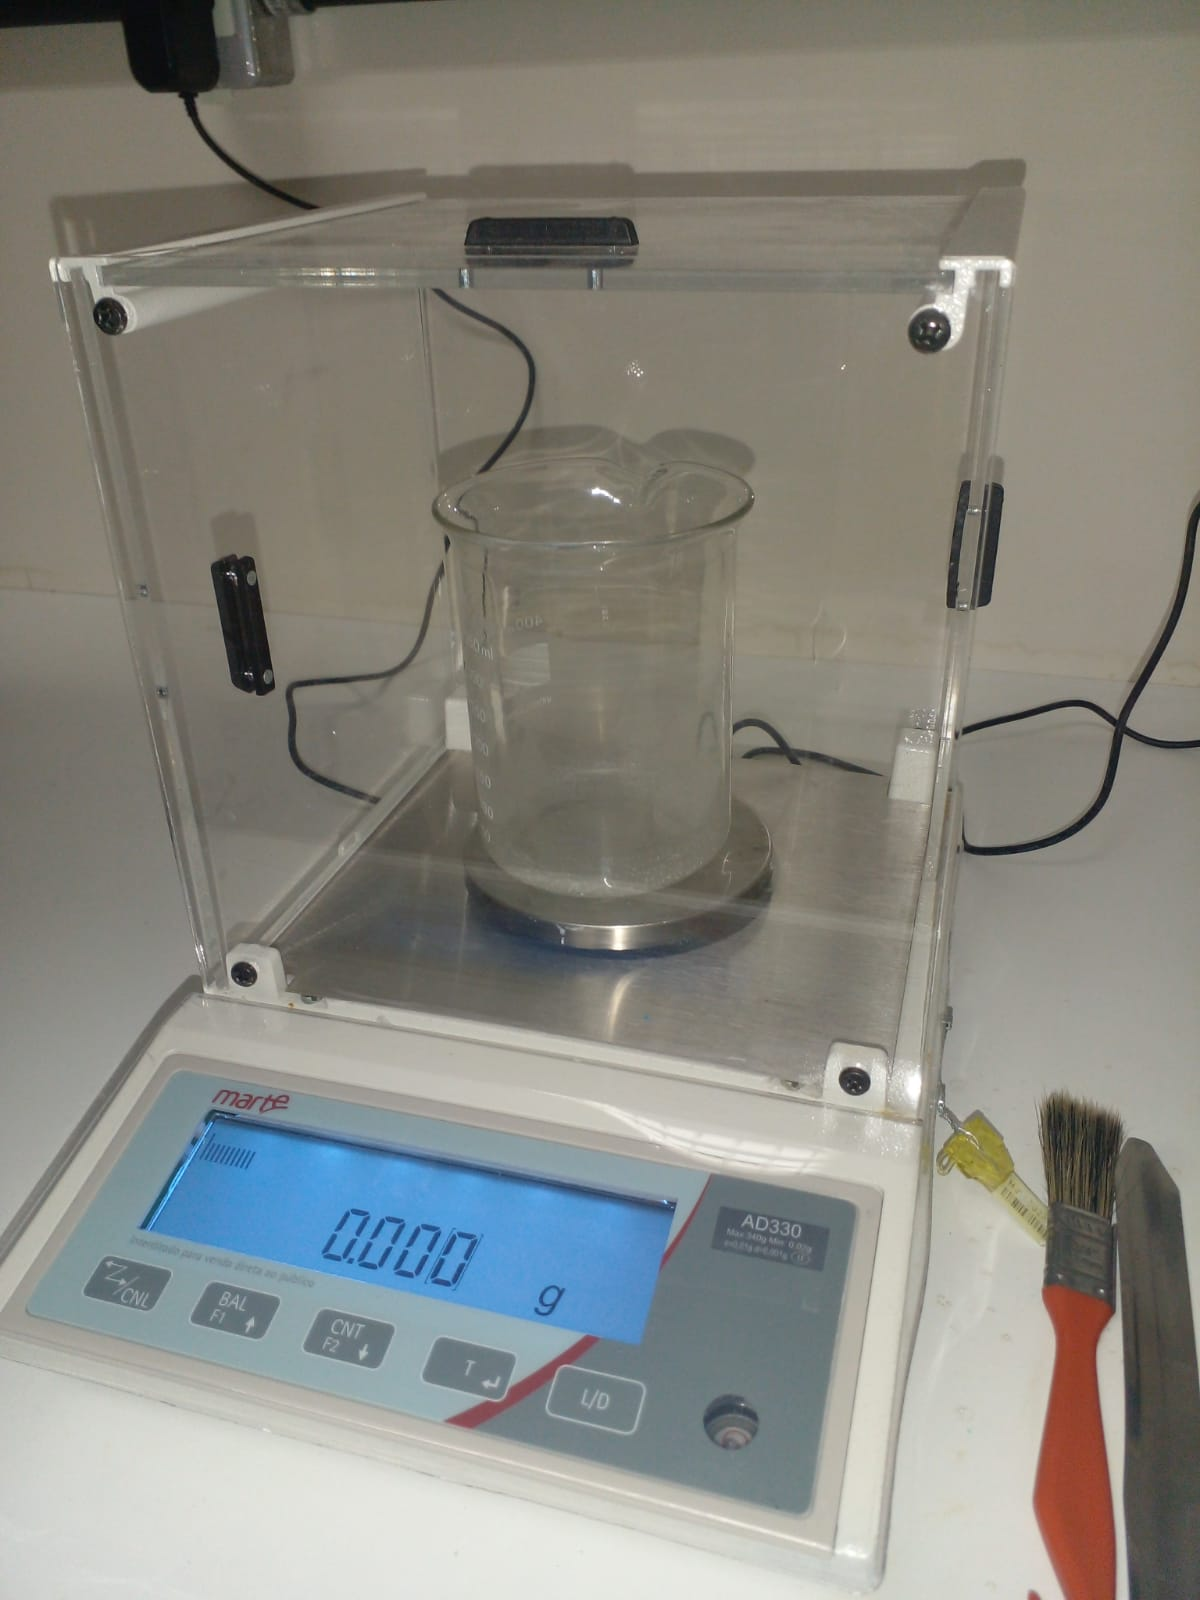
\includegraphics[scale=0.2]{03. preparo da balanca.jpeg}\\
            \textbf{Figura 1}: Preparo da balança\@.
        \end{center}
        \doublespacing

\newpage

        \indent O preparo da solução iniciou com a quantificação da massa, que no caso foi de $2.521g$, de sulfato de cobre II\@.\\

        \begin{center}
            \parbox{7cm}{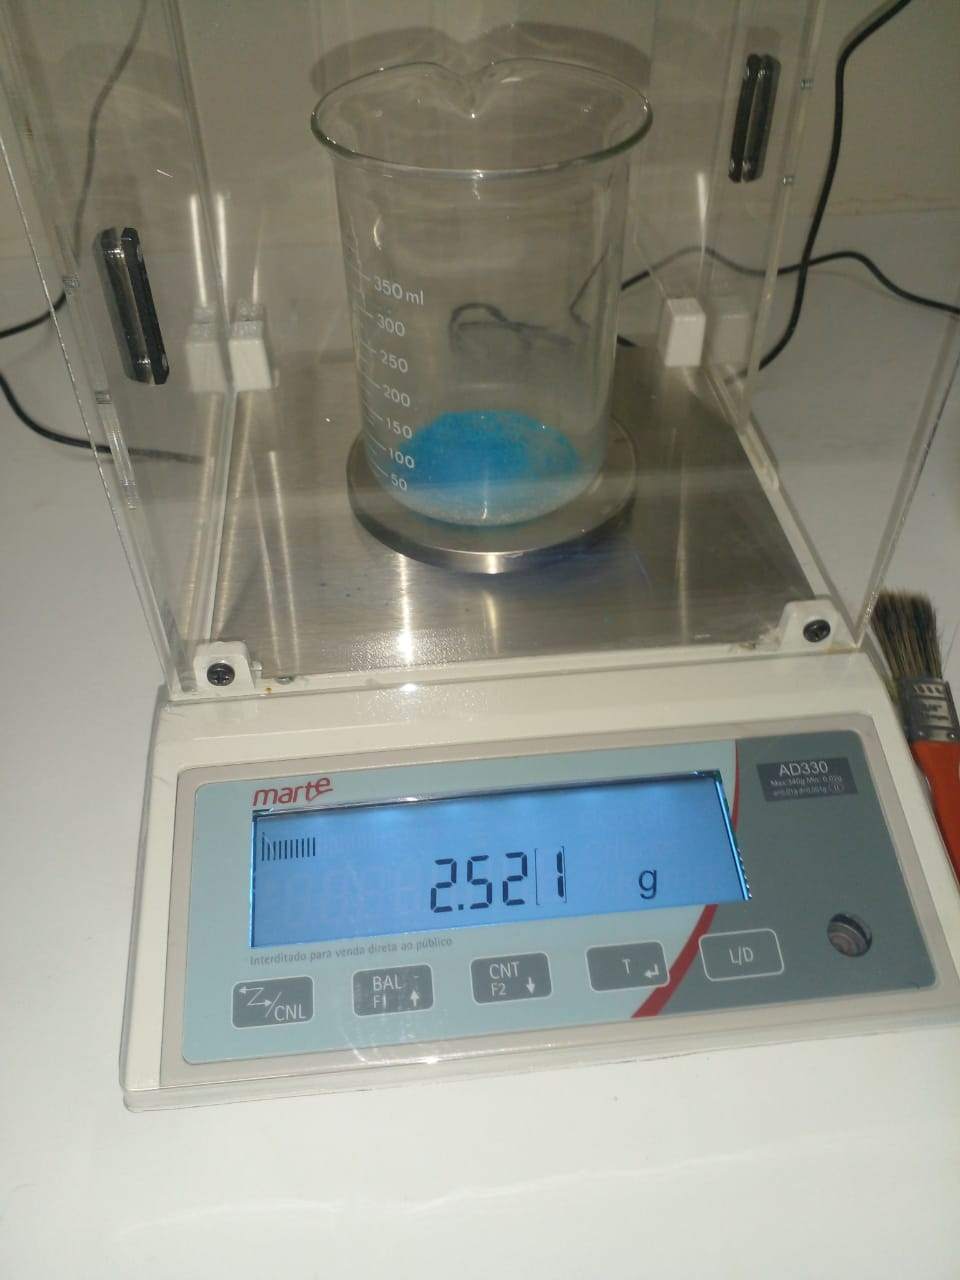
\includegraphics[scale=0.2]{02. massa_utilizada.jpeg}}\\
            \singlespacing
            \textbf{Figura 2}: Massa de sulfato de cobre II\@.
        \end{center}
        \doublespacing

        \indent Após a quantificação da massa, foi necessário preparar o balão volumétrico, o Funil e a Pisseta com água destilada\@.
        É necessário verificar a presença de umidade na vidraçaria utilizada, uma vez que tal condição pode afetar o procedimento\@.\\
        Podemos verificar na imagem a seguir que o Funil e o balão estavam secos, e a Pisseta contendo $200ml$ de água destilada\@: \\

        \begin{center}
            \parbox{7cm}{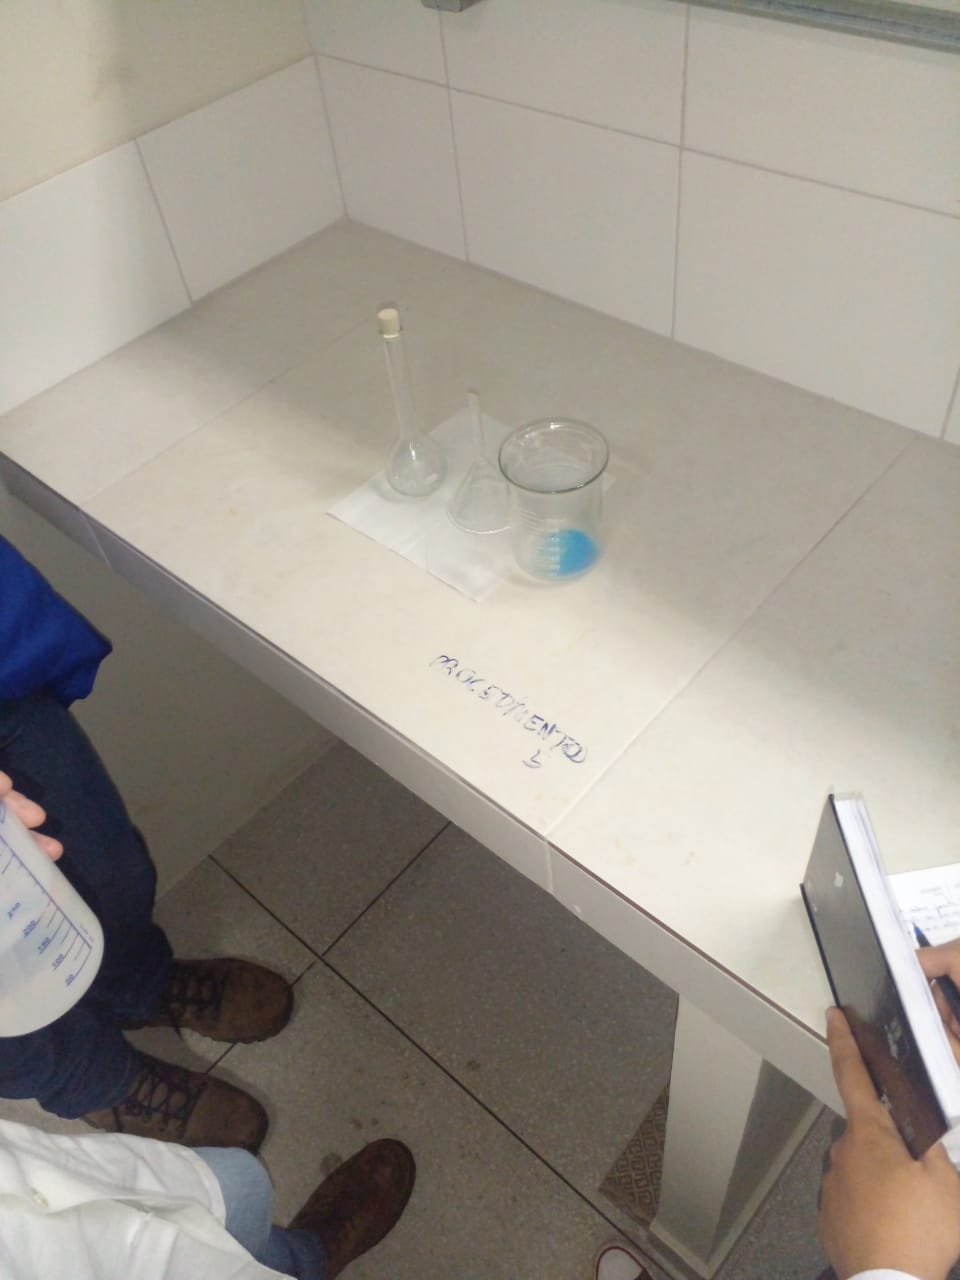
\includegraphics[scale=0.2]{01. instrumentos utilizados.jpeg}}\\
            \singlespacing
            \textbf{Figura 3}: Preparação do balão volumétrico\@.
        \end{center}
        \doublespacing

        \indent Logo após a preparação dos instrumentos, foi adicionado água destilada no becker para a solubilização do sulfato de cobre II,
        onde este foi agitado até que fosse totalmente solubilizado\@.
        verificou-se também, o encaixe do funil com o bocal do balão volumétrico, para que este não fosse totalmente vedado durante a
        adição do concentrado de sulfato de cobre II\@.\\

        \begin{center}
            \begin{tabular}{c c}
                \parbox{7cm}{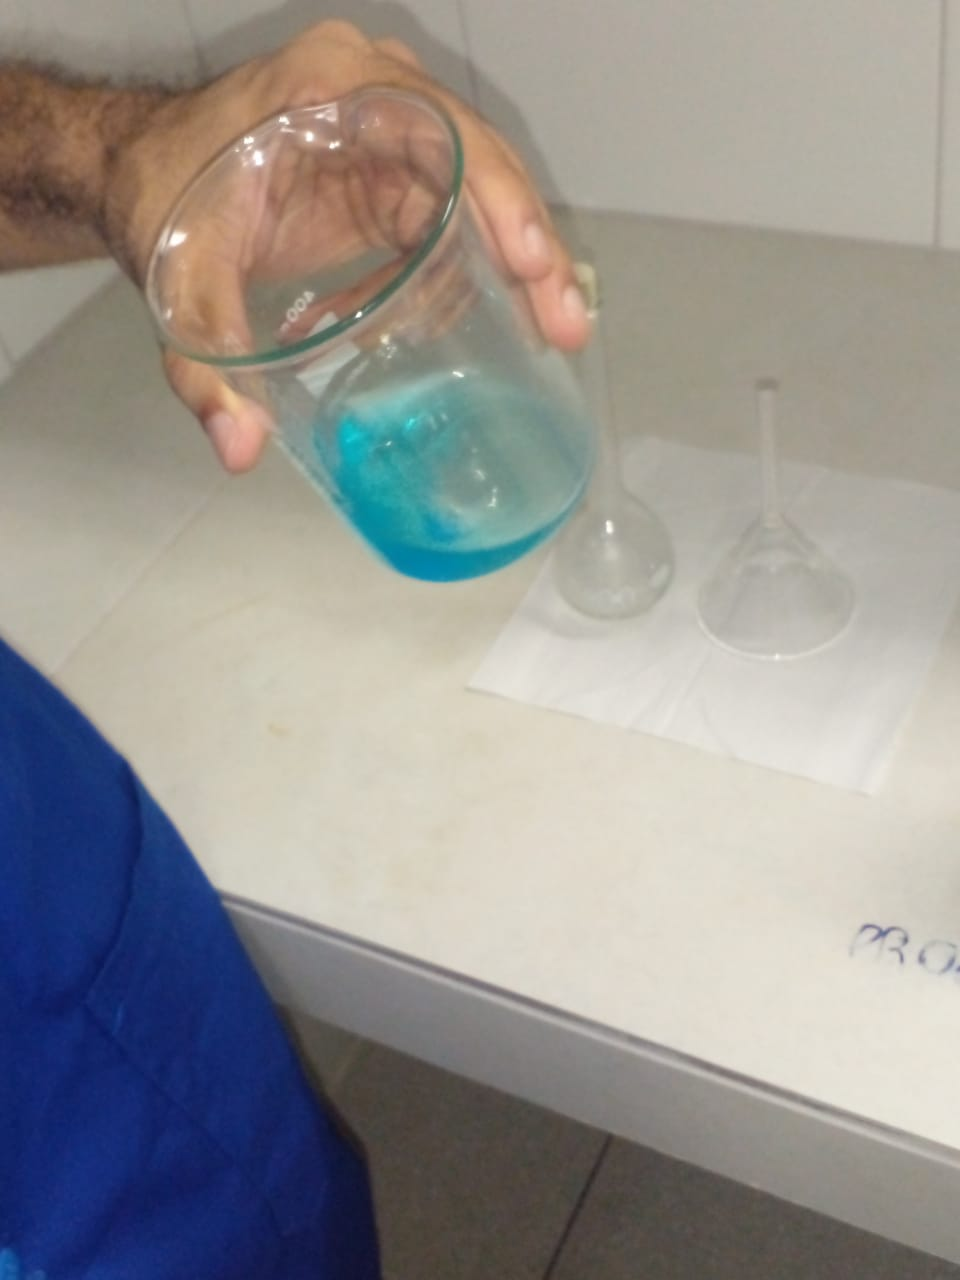
\includegraphics[scale=0.2]{05. solubilizacao.jpeg}}
                & \parbox{7cm}{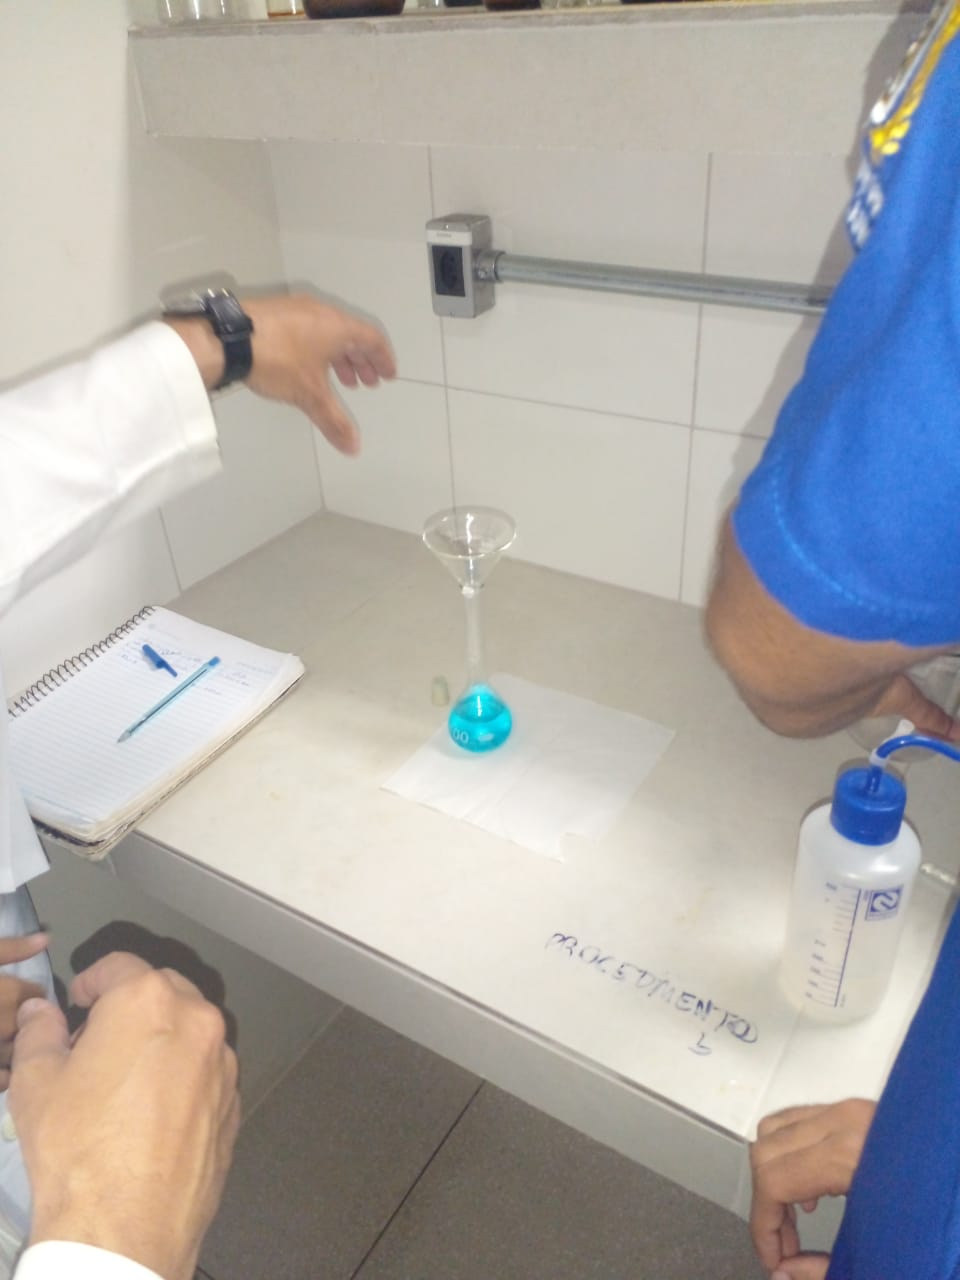
\includegraphics[scale=0.2]{04. preparo do balao.jpeg}}\\
                \\
                \textbf{Figura 4}: Solubilização do sulfato de cobre II\@.
                & \textbf{Figura 5}: Preparo do balão volumétrico\@.\\
            \end{tabular}
        \end{center}
        \doublespacing







        \begin{pycode}
            from sympy import *
            import pandas as pd

            mass = 2.521 # [g] CUSO4.5H2O
            molar_CUSO4 = 249.6850 # [g/mol] CUSO4.5H2O
            molar_H20 = 18.01528 # [g/mol] H20
            vol_H20 = 0.1 # [L] H2O
            rho_H20 = 1000 # [g/L] H20

            def int(theIntegrand,var):
                var  = symbols(var)
                anti = integrate(theIntegrand,var)
                return latex(anti)

            df = pd.Series({
                'Massa de CUSO4.5H2O [g]': mass,
                'Massa Molar de CUSO4.5H2O [g/mol]': molar_CUSO4,
                'Volume de Solvente (H20) [L]': vol_H20,
                'Mols de CUSO4.5H2O [mols]': mass/molar_CUSO4,
                'Mols de H20 [mols]': vol_H20 * rho_H20 / molar_H20
            })
            df = df.to_frame()




        \end{pycode}
        The result of integrating $\int \frac{1}{\sqrt{ 1+x }} \, dx$ is given by $\py{int("1/(1+x)**(1/2)","x")}$

            Here is some list of integrations to do

            \begin{align*}
            \int \frac{1}{\sqrt{ 1+x }} \, dx &=  \py{int("1/(1+x)**(1/2)","x")} \\
            \int \sin x \, dx &=  \py{int("sin(x)","x")} \\
            \int x \sin x \, dx &=  \py{int("x*sin(x)","x")} \\
            \int x^2 \sin x \, dx &=  \py{int("x**2 * sin(x)","x")} \\
            \int x e^{2 x} \, dx &=  \py{int("x*exp(2*x)","x")} \\
            \int \frac{1}{1+u} \, du &=  \py{int("1/(1+u)","u")} \\
            \end{align*}


\end{document}